\subsection{Состояние гонки}

\begin{frame}
	\tableofcontents[currentsection,currentsubsection]
\end{frame}

\begin{frame}{Демо гонки-1}
	Демо: \texttt{03-writeln-single}, \texttt{04-writeln-single}

	Valgrind не помогает.
\end{frame}

\begin{frame}{Состояние гонки: повезло}
	\svgimg{race-writeln-ok}
\end{frame}

\begin{frame}{Состояние гонки: не повезло}
	\svgimg{race-writeln-bad}
\end{frame}

\begin{frame}{Объяснение}
	\begin{itemize}
		\item
			Потоки выполняют команды <<одновременно>>.
			Если есть доступ к общему ресурсу (экран), то порядок не определить.
		\item
			Поэтому символы выводятся вперемешку.
		\item
			\textit{Состояние гонки} (\textit{race condition}) "--- это когда результат работы зависит от того, в каком порядке потоки выполняли команды.
		\item
			Самая популярная ошибка у начинающих.
		\item
			Операция называется \textit{атомарной}, если она всегда выполняется <<за один такт>>,
			то есть другие потоки не видят её частично выполненной.
		\item
			\t{writeln} выше не атомарна.
	\end{itemize}
\end{frame}

\begin{frame}{Демо гонки-2}
	Демо: \texttt{05-counter.cpp}, \texttt{06-even-counter.cpp}

	Важно: оптимизации отключены! (почему "--- на следующей лекции).

	Valgrind не помогает.
\end{frame}

\begin{frame}{Объяснение}
	Возможная последовательность действий:
	\begin{itemize}
		\item Основной поток: \t{if (data \% 2 == 0)} $\to \t{true}$.
		\item Второй поток: \t{data++}.
		\item Основной поток: \t{printf}.
	\end{itemize}
	Как исправить?
	\pause
	\begin{itemize}
		\item Можно на каждой итерации записать значение \t{data} в локальную \t{data\_snapshot} (снимок) и работать с ним.
		\item Работает только если чтение одной переменной атомарно.
		\item Не работает, если у нас много переменных мы не можем сделать атомарный снимок (классическая задача).
		\item Демо: \texttt{07-even-counter-snapshot.cpp}
	\end{itemize}
\end{frame}

\begin{frame}{Иллюстрация}
	\begin{center}
		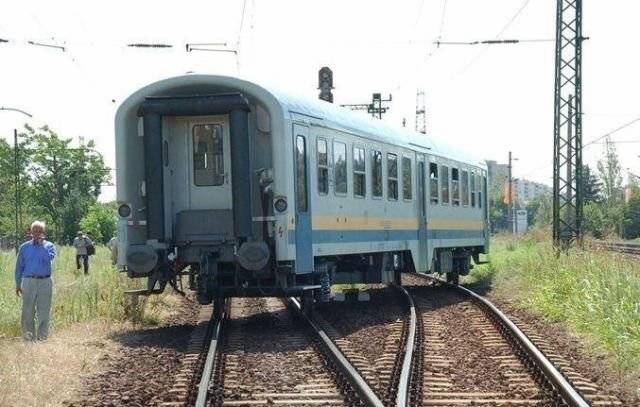
\includegraphics[scale=0.6]{race-condition.jpg}
	\end{center}
\end{frame}

\subsection{Гонка данных}
\begin{frame}{Демо гонки-3}
	Демо: \texttt{08-two-threads.cpp}

	Valgrind, внезапно, помогает (как и thread sanitizer).
\end{frame}

\begin{frame}[fragile]{Состояние гонки: повезло}
	\svgimg{race-two-inc-good}
\end{frame}

\begin{frame}[fragile]{Состояние гонки: не повезло}
	\svgimg{race-two-inc-bad}
\end{frame}

\begin{frame}{А что вообще атомарно?}
	\begin{center}
		
\includegraphics[scale=0.4]{absolutely-nothing.jpg}
	\end{center}

	Даже в Python или Java.
\end{frame}

\begin{frame}{Полезные советы}
	\begin{itemize}
		\item
			Что атомарно "--- очень сильно зависит от платформы, языка и ключей компиляции
			(<<модель памяти>>).
		\item Не пытайтесь угадать.
		\item Не пытайтесь самостоятельно писать код, зависящий от атомарности.
		\item В некоторых языках бывает \t{AtomicInteger} и похожие структуры.
		\item За ними тоже надо аккуратно следить, обычно не используют.
		\item Мораль из Rust:
			\begin{itemize}
			\item Несколько потоков, читающих одну переменную "--- окей
			\item Если кто-то пишет в переменную, то никто другой не может её читать
			\end{itemize}
	\end{itemize}
\end{frame}
